\documentclass[conference]{assets/latex/IEEEtran}
\IEEEoverridecommandlockouts

\usepackage{amsmath,amssymb,amsfonts}
\usepackage{graphicx}
\usepackage{textcomp}
\usepackage{xcolor}
\usepackage[backend=biber,style=numeric]{biblatex}
\addbibresource{assets/latex/report.bib}

\graphicspath{{assets/latex/}}

\begin{document}

\title{CS6524 Computer Vision Lab 3:\\ Structure from Motion}

\author{\IEEEauthorblockN{Patrick Walsh}
\IEEEauthorblockA{23372176 \\ University of Limerick}}

\maketitle

\begin{abstract}
I built an incremental Structure from Motion (SfM) pipeline in Python and OpenCV and used it to
reconstruct a trainer from two iPhone videos: one where I walked the camera around the shoe, and
one where the camera stayed still and the shoe spun on a stool. The pipeline tracks SIFT
keypoints, gets the relative motion from essential matrices, registers each new frame with PnP,
corrects drift with windowed bundle adjustment and finally builds a dense cloud with
semi-global block matching. The moving-camera video worked well, with every frame registered and
a sub-pixel reprojection error. The spinning-object video was much harder because the shoe only
covers a small part of the frame and the stool turned unevenly. I also tested how sensitive the
result is to a wrong focal length and to skipping undistortion.
\end{abstract}

\section{Data and Calibration}

Both videos were filmed on an iPhone 13 in portrait at $720\times1280$ and 30\,fps. The object
is a worn Adidas trainer sitting on a small black stool in a study room. In video $a$ (21\,s) I
walked one full lap around the stool. In video $b$ (29\,s) the phone was propped up and I turned
the stool by hand. The first 6.5\,s of $b$ were cut because nothing moved yet. Both videos were
re-encoded with H.264 to stay under 5\,MB.

For the intrinsics I reused my own phone's calibration from Lab~2 (Cam~01), which was done at
$360\times640$: $f_x=453.7$, $f_y=452.7$, $c=(188.8, 318.0)$. Since the new videos are twice that
size, $K$ is scaled by the ratio of the widths before use. For distortion I only kept $k_1$,
$p_1$ and $p_2$ and set $k_2=k_3=0$. In Lab~2 we found that $k_2$ and $k_3$ were badly overfit
($k_3=-115$) because the checkerboard only ever covered the middle of the frame. Using them here
would bend the edges of every frame, so dropping them was the safer choice.

\section{Methodology}

\subsection{Frame selection and tracking}
For video $a$ I keep every 8th frame, which gives 80 frames that cover the whole lap, and process
them at $360\times640$. Video $b$ needed more care. The shoe only fills the bottom third of the
portrait frame, so I keep it at full resolution and crop to the band between 55\% and 97\% of
the height. When cropping I shift the principal point of $K$ by the crop offset, so the
intrinsics stay correct. Because I turned the stool in pushes, many frames barely moved. To deal
with this I added a keyframe step: a frame is only kept once the fastest 10\% of
Lucas--Kanade corner tracks have moved at least 12\,px since the last kept frame. This left 73
keyframes.

In each kept frame I detect up to 3000 SIFT keypoints. Consecutive frames are matched with a
mutual nearest-neighbour check and Lowe's ratio test (0.75), and outliers are removed with a
fundamental-matrix RANSAC. Matches are then chained into tracks, so a point seen in frames 3, 4
and 5 becomes one track with three observations. For video $b$ I also drop any match that moves
less than 3\,px. Otherwise the static wall behind the stool wins the RANSAC vote and the shoe is
thrown away as an outlier.

\subsection{Two-view initialisation}
The first camera is the world origin. I try the pairs $(0,k)$ for $k=1\dots4$, estimate the
essential matrix with MAGSAC, recover $R$ and $t$ with \texttt{recoverPose} and triangulate the
shared tracks with the linear (DLT) method. A point is only accepted if it is in front of both
cameras, reprojects within 3\,px in both views and has a triangulation angle above $1^\circ$.
The pair with the most accepted points wins. I had to add this search because with only frames
0 and 1 the RANSAC would sometimes land on a wrong solution with almost no valid points.

\subsection{Extending to N frames}
For every new frame I still compute the essential matrix with the previous frame, but the
translation from $E$ has no scale, so chaining them would give every step a length of one. The
absolute pose therefore comes from PnP: the tracks that already have a 3D point give 2D--3D
pairs, and \texttt{solvePnPRansac} plus a Levenberg--Marquardt refine gives a pose in the same
scale as the existing map. Only when PnP fails do I fall back to chaining the essential-matrix
motion, reusing the length of the previous step. New tracks are then triangulated against the
oldest registered frame (up to 5 back) that also sees them, which gives a wider baseline than
always using the previous frame.

To stop the error from building up, a bundle adjustment runs every 5 frames over the last 8
frames. It jointly refines those camera poses and every point they see by minimising the
reprojection error with \texttt{scipy.optimize.least\_squares}, a sparse Jacobian and a Huber
loss so a few bad matches cannot dominate. A final global bundle adjustment runs over all frames,
and points that still reproject worse than 6\,px anywhere are removed.

\subsection{Dense reconstruction}
Once every frame has a pose, I take every second frame and its neighbour as a stereo pair.
Since the relative pose is known, \texttt{stereoRectify} can align the two images, and SGBM gives
a disparity for nearly every pixel. These are back-projected to 3D, moved into the world frame
and kept only if their depth falls in the range covered by the sparse points. To average across
frames, all points go into a voxel grid with cells 0.5\% of the scene size. Each voxel becomes
the mean position and colour of its points, and voxels hit fewer than twice are dropped as noise.

\subsection{Sensitivity analysis}
For both videos I ran the full pipeline with $f_x$ and $f_y$ multiplied by 0.8, 1.0 and 1.2, both
with and without undistortion, giving 12 runs. The scaled $K$ is used everywhere, including in
the undistortion itself, so a run simulates a camera that was calibrated wrongly.

\section{Results}

\begin{table}[t]
\caption{Results of the 12 runs (u = undistorted, d = distorted). Error is the mean reprojection error over all registered frames.}
\begin{center}
\begin{tabular}{lcccc}
\hline
Run ($f$ factor) & Frames & Sparse pts & Dense pts & Error (px) \\
\hline
$a$, $0.8$, u & 80 & 8261 & 137600 & 0.73 \\
$a$, $1.0$, u & 80 & 10676 & 220887 & 0.32 \\
$a$, $1.2$, u & 80 & 8346 & 290175 & 0.61 \\
$a$, $0.8$, d & 80 & 5343 & 43854 & 0.93 \\
$a$, $1.0$, d & 80 & 8407 & 143691 & 0.58 \\
$a$, $1.2$, d & 80 & 10399 & 404708 & 0.22 \\
\hline
$b$, $0.8$, u & \multicolumn{4}{c}{failed to initialise} \\
$b$, $1.0$, u & 73 & 2103 & 214589 & 0.59 \\
$b$, $1.2$, u & \multicolumn{4}{c}{failed to initialise} \\
$b$, $0.8$, d & \multicolumn{4}{c}{failed to initialise} \\
$b$, $1.0$, d & 73 & 1658 & 15048 & 0.87 \\
$b$, $1.2$, d & 73 & 1513 & 90396 & 0.89 \\
\hline
\end{tabular}
\label{tab:results}
\end{center}
\end{table}

\begin{figure}[t]
\centerline{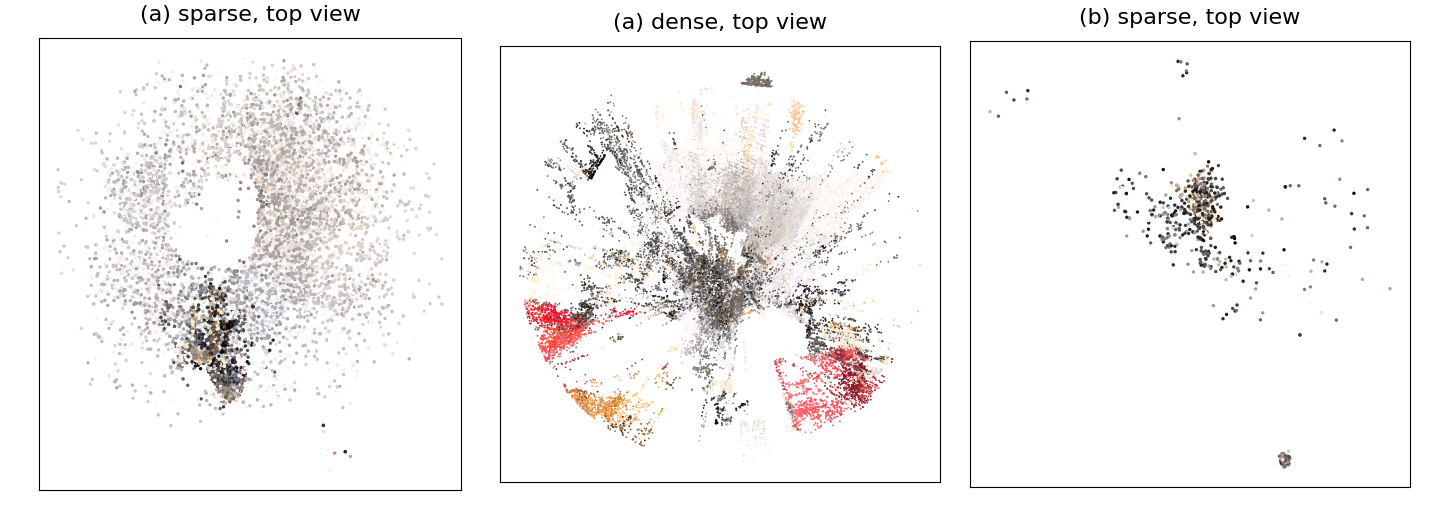
\includegraphics[width=\columnwidth]{fig_clouds.png}}
\caption{Top views of the reconstructions with the original focal length and undistortion. Left:
sparse cloud of video $a$, with the shoe and stool as the dark cluster inside a ring of floor
points. Middle: dense cloud of $a$, where the room around the lap (including the red chairs) is
visible. Right: sparse cloud of $b$, a small cluster on the shoe.}
\label{fig:clouds}
\end{figure}

Table~\ref{tab:results} shows all 12 runs. Video $a$ registered all 80 frames in every run. Video $b$ only
initialised in three of its six runs, and when it worked it kept all 73 keyframes.
Fig.~\ref{fig:clouds} shows what the clouds look like from above. For $a$ the full lap is clear:
the shoe and stool sit in the middle and the floor and furniture of the room spread out around
them. The cloud for $b$ is much smaller and sparser, with about 2000 points against more than
10000 for $a$.

\section{Discussion and Failure Analysis}

\textbf{Focal length.} For video $a$ with undistortion, the correct focal length gives
the lowest error (0.32\,px). Scaling it by 0.8 or 1.2 roughly doubles the error. The pipeline
never changes $K$, so a wrong focal length has to be absorbed by the poses and the points, and
the bundle adjustment cannot fully hide it. Lowering $f$ hurt the most, and it also gave the
fewest points, because a short focal length makes the rays spread out more and more triangulated
points fail the reprojection check.

\textbf{Undistortion.} Skipping undistortion with the right focal length almost doubled the
error for $a$ (0.32 to 0.58\,px), which shows that even the mild barrel distortion of the iPhone
($k_1=-0.12$) matters. The odd result is $a$ at $f\times1.2$ without undistortion, which has the
lowest error of all (0.22\,px). My best explanation is that a longer focal length partly mimics
the barrel distortion, since both change how quickly points move away from the centre of the
image. This is also a reminder that reprojection error only measures how consistent the model is
with itself. A model can fit its own tracks very well and still have the wrong shape, for example
with the depth stretched. Without a ground-truth measurement of the shoe I cannot say which run
is really the most accurate.

\textbf{Dense point counts.} The number of dense points rises with the focal length in both the
undistorted and distorted runs. I do not think this means better quality. A longer focal length
stretches the scene in depth, so the depth window taken from the sparse points gets wider and
more SGBM pixels pass the filter. Many of these extra points are the room behind the shoe, not
the shoe itself.

\textbf{Why video $b$ is harder.} Three of the six $b$ runs could not even initialise. A
spinning object in front of a still camera is the same problem in theory as walking around it,
but in practice my video made it much harder. The shoe only covered a small strip of the frame,
and its black upper has little texture, so I only got about 46 good matches per frame pair,
compared with over 300 for $a$. Most features sat on the brick wall, which had to be thrown away
with the 3\,px motion filter. I also turned the stool by hand, so the motion came in bursts, and
the keyframe step was needed just to get usable pairs. With so few matches, the first essential
matrix is fragile. With a wrong $K$ it often found fewer than 10 points that passed the checks,
and the run stopped. Even in the runs that worked, PnP failed on several frames and the
pipeline had to fall back to chaining essential-matrix poses. In my local tests the global bundle
adjustment still left an RMS error in the tens of pixels before outlier removal. The low mean
error in Table~\ref{tab:results} is measured after the bad points are removed, so it makes $b$
look better than it is. Overall, video $a$ is a success and video $b$ is only a partial one: the
pipeline produces a cloud of the shoe, but it is sparse and not reliable when the intrinsics are
wrong.

\section{Improvements With More Time}

The biggest gain would come from better data for video $b$: a proper turntable for a smooth spin,
the phone closer so the shoe fills the frame, and a plain backdrop instead of a brick wall. On
the algorithm side, I would add loop closure. After a full lap the last frames see the same side
of the shoe as the first ones, and matching them would let the bundle adjustment pull the two
ends of the trajectory together. I would also recalibrate the phone with the board moved into
the corners of the frame, so that $k_2$ and $k_3$ could be trusted and the undistortion
comparison would mean more. Finally, the dense step treats every stereo pair separately, and a
multi-view method that checks depth consistency across several frames would remove most of the
floating noise around the shoe.

\nocite{foundationsCVbook}
\printbibliography

\end{document}
